\documentclass[11pt,letterpaper]{article}

\usepackage[letterpaper,margin=0.8in,nohead]{geometry}

\usepackage[colorlinks]{hyperref}
\usepackage{url}
\usepackage{breakurl}

\hypersetup{
    colorlinks,
    linkcolor={red},
    citecolor={red},
    urlcolor={blue}
}

\usepackage{verbatim}
\usepackage{fancyvrb}
\usepackage{scrextend}
\usepackage{enumitem}
\usepackage{url}

\usepackage{caption}
\usepackage{graphicx}
\usepackage{subcaption}

\usepackage{changepage}   % for the adjustwidth environment

\newenvironment{answer}{\em \color{blue} \begin{adjustwidth}{1cm}{1cm}}{\end{adjustwidth}}

% math
\usepackage{amsthm,amsmath}
\usepackage{amsfonts}

\newcommand{\mc}[1]{\mathcal{#1}}	% Mechanisms / Algorithms
\newcommand{\rv}[1]{\mathbf{#1}}    % Random variable

\newcommand{\pr}[1]{\mathrm{Pr}\{#1\}} % Probability

\newtheorem{corollary}{\bf Corollary}%[theorem]
\newtheorem{lemma}{\bf Lemma}%[theorem]
\newtheorem{definition}{\bf Definition}%[section]

\newtheorem{observation}{\bf Observation}%[theorem]

\include{macros-v2}

% load cleveref last!
\usepackage[capitalise]{cleveref}

\crefname{observation}{Observation}{Observations}


\begin{document}

\title{EN3240: Embedded Systems Engineering \\Assignment 1 --- Modeling \& Specification}

%% This is an individual assignment!!
%% TODO: put your name and index number here!
\author{Name: Thalagala B. P. \\ Index No: 180631J}

\maketitle

\begin{center}
	\color{red}\bf This is an individual assignment! \\ Due Date: 28 August 2022 by 11.59 PM
\end{center}

\section*{Instructions}
%

Please read the instructions and questions carefully. Write your answers directly in the space provided. Compile the tex document and submit the resulting PDF. This is an individual assignment. You are not allowed to take or give any help in completing this assignment.

When drawing images, you may draw them by hand, take a photo and add that as a Figure in LaTeX. Please avoid this option unless you have excellent handwriting and drawing capability!

%%%%%%%%%%%%%%%%%%%%%%%%%%%%%%%%%
%%%%%%%%%%%%%%%%%%%%%%%%%%%%%%%%%

\newpage
\section*{Problem : Petri Nets (10 Points)}

{\bf Draw} a  condition/event Petri  net  model  for  the  following  library  system. Assume  that there  are three  desks  available  to  users  in  a  library: the  reception  desk,  the  collection  desk  and  the  return  desk.  All the  books  are kept in the warehouse and have a scan code.  The process goes as follows. A user goes to the reception desk to borrow a book. If the book is available in the warehouse, it will be fetched and the scan code will be scanned. The user can get the book in the collection desk. When the user finishes reading the book, it will be returned to the return desk. After the scan code  is  scanned  again,  the  book  is  accepted  and  replaced  in  the  warehouse. Note  that  there  is  only  one  scanner  in  the library. Therefore,  it  is  shared  between  the  collection  desk  and  the  return  desk.  Moreover,  assume  that  there  are  three employees in the library –one works full-time in the reception desk, the second one works full-time in the warehouse, and the third employee works both in the collection desk and the return desk (s/he cannot be in both desks at a time). In your design, assume the basic condition/event model where a transition is activated when there is one token in each of the input places, and after activation one token is placed in each of the output places (no need to show any number on the arcs). In your  design,  please  show  the  following  four  transitions  (events):  receive  book,  scan  book,  return  book,  and  warehouse transfer.  Please  use  the  following seven places  (tokens)  in  your  design:  user  1,  user  2, book, scanner,  employee  1, employee 2 and employee 3. Please use additional places/tokens/transitions, if needed. Also, the name can be different (if needed), e.g., “employee 1 at reception desk” or “user 2 at return desk”. Place tokens  in  your  Petri  net  to  show  the scenario when there are two users in the library –one in the reception desk to borrow a book and the other in the return desk to return a book.

\pagebreak
\section*{Solution}
\begin{figure}[!h]
	\centering
	\fbox{
	\includegraphics[scale= 0.9]{Figures/library.png}}
	\caption{Condition/Event Petri  net  model  for  the library  system, showing the scenario when there are two users in the library –one in the reception desk to borrow a book and the other in the return desk to return a book}
\end{figure}

\end{document}
